\documentclass[conference]{IEEEtran}
\IEEEoverridecommandlockouts
% The preceding line is only needed to identify funding in the first footnote. If that is unneeded, please comment it out.
\usepackage{cite}
\usepackage[ngerman]{babel}
\usepackage[utf8]{inputenc}
\usepackage{amsmath,amssymb,amsfonts}
\usepackage{algorithmic}
\usepackage{graphicx}
\usepackage{textcomp}
\usepackage{xcolor}
\usepackage{listings}


\definecolor{pblue}{rgb}{0.13,0.13,1}
\definecolor{pgreen}{rgb}{0,0.5,0}
\definecolor{pred}{rgb}{0.9,0,0}
\definecolor{pgrey}{rgb}{0.46,0.45,0.48}
\lstset{language=Java,
	showspaces=false,
	showtabs=false,
	breaklines=true,
	tabsize=2,
	showstringspaces=false,
	breakatwhitespace=true,
	commentstyle=\color{pgreen},
	keywordstyle=\color{pblue},
	stringstyle=\color{pred},
	basicstyle=\ttfamily
}


\usepackage{url}
\def\BibTeX{{\rm B\kern-.05em{\sc i\kern-.025em b}\kern-.08em
		T\kern-.1667em\lower.7ex\hbox{E}\kern-.125emX}}
\begin{document}
	
	\title{Computational Geometry - Abgabe 4}
	
	\author{\IEEEauthorblockN{1\textsuperscript{st} Bartolovic Eduard}
		\IEEEauthorblockA{\textit{Hochschule München} \\
			München, Deutschland \\
			eduard.bartolovic0@hm.edu}
	}
	
	\maketitle
	
%\begin{abstract}	
%\end{abstract}

	\section{Konvexe Hülle}
	Für die Berechnung der konvexen Hülle wurde das Programm \textit{qhull} \cite{b2} verwendet. \textit{qhull} verwendet den Quickhull Algorithmus um die konvexe Hülle zu berechnen. \textit{qhull} lässt sich per Kommandozeile ansprechen. Ein Beispiel für einen Aufruf:
	\begin{lstlisting}[basicstyle=\small]
	rbox 3 D2 | qconvex s o TO result
	\end{lstlisting}
	Der Befehl \textit{rbox} generiert eine gewisse Anzahl an Punkten in einer definierten Dimension. Der Befehl \textit{qconvex} berechnet die konvexe Hülle. Mit einer Pipe können die Punkte direkt \textit{qconvex} übergeben werden.\\
	\section{Laufzeit von \textit{qhull}}
	Es wurde die Laufzeit von \textit{qhull} untersucht. Hierbei wurden verschiedene Konfiguration bezüglich Anzahl und Dimension getestet. Um den Einfluss von Ausreißern zu reduzieren, wurde das mittel aus fünf Durchläufen gebildet. Um das Problem etwas zu automatisieren, entwickelte ich ein Batchfile welches \textit{qhull} mit definierten Konfigurationen automatisch fünf mal gestartet hat. Die Anzahl der Punkte, die getestet worden sind:
	\begin{itemize}
		\item 1000
		\item 10000
		\item 100000
		\item 500000
		\item 1000000
		\item 2500000
		\item 5000000
		\item 7500000
		\item 10000000
		\item 20000000
	\end{itemize}
	Jede Punkteanzahl wurde mit den Dimensionen 2 bis 8 getestet.\\
	\textit{Qhull} ist auf Windows nur für 32 Bit kompiliert. Dies resultiert darin, dass Qhull nur 4 GB Arbeitsspeicher allokieren kann. Deshalb schlägt ab der Dimension 5 bei einer höheren Punktezahl das Programm fehl. Da aber die Laufzeiten extrem ansteigen, ist dies nicht weiter tragisch.\\
	Die Ergebnisse der Messungen sind in den beiden Abbildungen \ref{figure_1} und \ref{figure_2} zu sehen.\\
	\begin{figure}[h!]
		\begin{center}
			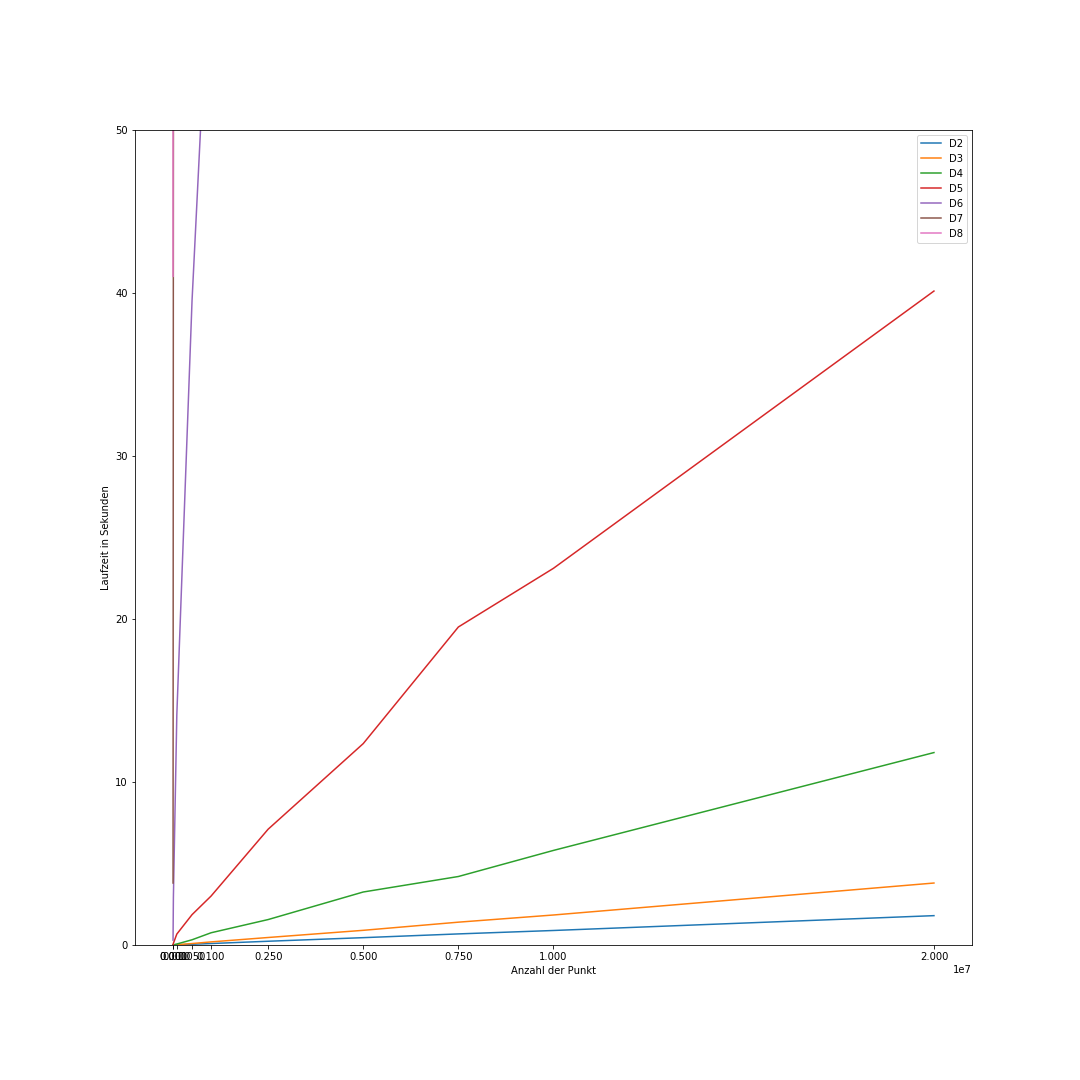
\includegraphics[width=7cm]{Laufzeit.png}
			\caption{Messung der Laufzeit abhängig zur Anzahl der Punkte und Dimensionen}
			\label{figure_1}
		\end{center}
	\end{figure}
	\begin{figure}[h!]
		\begin{center}
			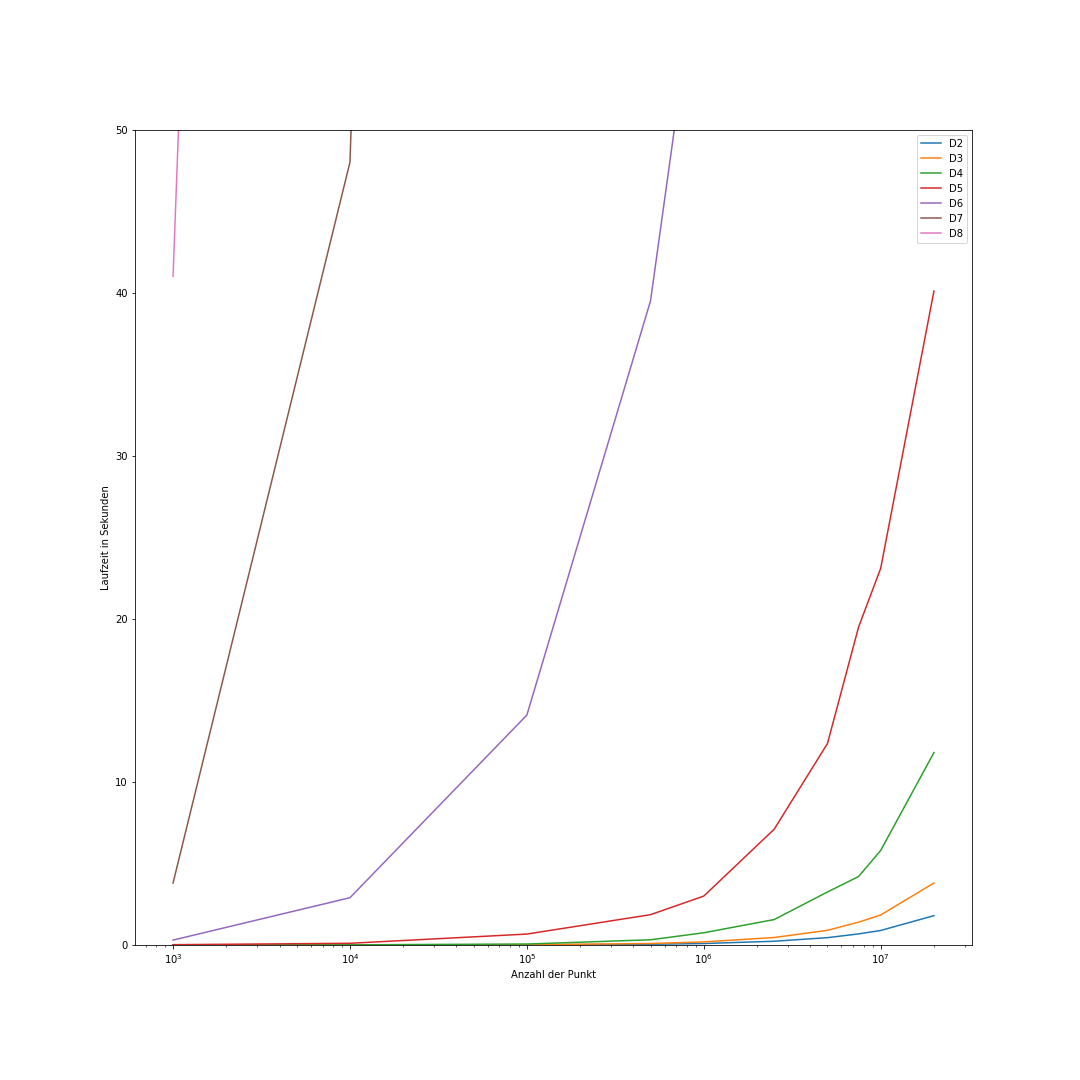
\includegraphics[width=7cm]{Laufzeitlog.png}
			\caption{Messung der Laufzeit abhängig zur Anzahl der Punkte und Dimensionen (X-Achse ist Log Skaliert)}
			\label{figure_2}
		\end{center}
	\end{figure}\\
	Wie gut in den Messungen zu sehen ist steigt der Aufwand mit Anzahl der Punkte und Dimensionen. Die Laufzeit steigt deutlicher mit der Dimension als mit den Punkten.\\
	Die gemessenen Laufzeitsteigerungen der Punkte entsprechen grob der durchschnittlichen Komplexität von Quickhull mit $\mathcal{O}(n * \log(v))$ bei Dimensionen von 2 und 3. $n$ entspricht der Anzahl der Input Punkte. $v$ ist die Anzahl der Punkte der Konvexen Hülle.\\
	Ab einer Dimension von größer 3 steigt der Aufwand auf $\mathcal{O}(\frac{n*f_v}{v})$. $f_v$ sei die maximale Anzahl von Facetten für eine konvexe Hülle aus den Eckpunkten.\\
	In Abhängigkeit der Dimension wächst $f_v$ sehr schnell mit: \[\mathcal{O}(\frac{v^{\text{floor}(d/2)}}{\text{floor}(d/2)!})\]
	\cite{b3}
	
	\begin{thebibliography}{00}
		\bibitem{b2} http://www.qhull.org/html/qconvex.htm
		\bibitem{b3} http://www.geom.uiuc.edu/~bradb/qhull3.1/html/qh-in.htm
	\end{thebibliography}
	
	
	
	\section{Anhang}

	Batchfile zum Testen der Laufzeit von Q-Hull:
	\begin{lstlisting}[basicstyle=\tiny]
	rbox 5000000 D2 | qconvex s o TO result1
	rbox 5000000 D2 | qconvex s o TO result2
	rbox 5000000 D2 | qconvex s o TO result3
	rbox 5000000 D2 | qconvex s o TO result4
	rbox 5000000 D2 | qconvex s o TO result5
	\end{lstlisting}	

\end{document}
